Consider $\xi$ as
\begin{equation*}
	f(r) = \left\langle \sigma_j^z \sigma_{j+r}\right\rangle \propto e^{- r /\xi},
\end{equation*}
so we could estimate it numerically (fig. \ref{fig:raf}). We have finite $L$ that strongly affects $\xi$ estimation, but definitely something interesting happens at $h=\sub{h}{c}=1$.

 We know that
\begin{equation*}
	\frac{1}{\sub{E}{gap} }  \propto \frac{1}{\varepsilon_{k=0}} \propto  \xi^{z} \propto (h - \sub{h}{c})^{-\nu z},
\end{equation*}
and from \eqref{gap} at $k=0$ we have $\sub{E}{gap} \propto h-1$, than $\sub{h}{c}=1$ and $\nu z = 1$.

\begin{figure}[h]
    \centering
    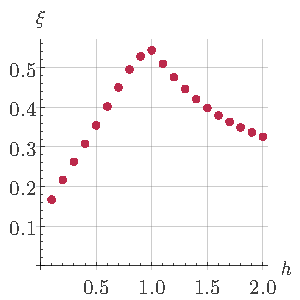
\includegraphics[width=0.25\textwidth]{imgs/3rad.pdf}
    \caption{Correlation radius $\xi$ as a function of external magnetic field $h$ at $L=20$, ground state}
    \label{fig:raf}
\end{figure}
